\documentclass[a4paper,11pt]{kth-mag}
\let\ifpdf\relax
\usepackage[T1]{fontenc}
\usepackage{textcomp}
\usepackage{lmodern}
%\usepackage[latin1]{inputenc}
\usepackage[swedish,english]{babel}
\usepackage{modifications}
\usepackage{amsmath}
\usepackage{ifpdf}
\usepackage[breaklinks=true]{hyperref}
\usepackage{breakcites}
\usepackage{pdfpages}
\newcommand{\textunderscript}[1]{$_{\text{#1}}$}
\usepackage[utf8]{inputenc}
\usepackage{cite}
%\usepackage{biblatex}
%\addbibresource{references.bib}
\newenvironment{italicquotes}
{\begin{quote}\itshape}
{\end{quote}}
\usepackage{graphicx}


%\usepackage{appendix} 
\title{Balancing Cube (working title)}
\subtitle{Control and design of reaction wheel balanced inverted pendulum}
\foreigntitle{Stabilisering med svänghjul}
\author{Mikael Sjöstedt \\ Alexander Ramm}
\date{May 2015}
\blurb{ Bachelor's Thesis in Mechatronics \vspace{1em} \\
\begin{tabular}{ll} 
Supervisor: Daniel Frede &  \\
Examiner:Martin Edin Grimheden \\ 
Approved: & TBA 2015-month-day
\end{tabular} }
\trita{TRITA xxx yyyy-nn}


\begin{document}

%
\includepdf[pages={1}]{kth-cover.pdf}
\clearpage

\frontmatter
\pagestyle{plain}
%\removepagenumbers
\pagenumbering{roman}
\maketitle
\selectlanguage{english}
\begin{abstract}
\addcontentsline{toc}{chapter}{Abstract}
This thesis is about implementing automated control and balance a simple construction using a reaction wheel commonly used in satellites...
\\ To be filled in:
\\	Problem
\\	Approach % (On the premiss of constructing a small box shaped robot components with desired properties were chosen....)
\\	Results
\\ 	Conclusion


%(The thesis is written in English and it has both a Swedish and an English \textit{Abstract} page. An English thesis has English \textit{Cover} and \textit{Title} pages. This template, which has no bookmarks or other automation features, defines the layout of a bachelor thesis in Machine Design (MF123X) or Industrial Engineering (MF105X).  The chapter structure that is presented here is just an example.
%The abstract is maximum one page long. The abstract page is followed by a blank page. The preceding title page, which preferably contains an illustrative picture, is also followed by a blank page. All chapters start at the top of a right hand page, i.e. a page with an odd number.) 
\end{abstract}
\cleardoublepage
\begin{foreignabstract}{swedish}
\addcontentsline{toc}{chapter}{Sammanfattning}
Projektet gick ut på att bygga en kub som kan balansera på en kant med hjälp av ett reaktionshjul. Dessutom sulle den undersökas huruvida det gick att förbättra reglersystemet
för cuben, så den klarade en större yttre störning. Ingengörsproblemet delades upp i mindre delproblem och kuben byggdes. Reglestystemet beräknades på formen "State space" och implementerades.
Från resultatet drogs slutsatserna att...
\\


%Examensarbetet skrivs på engelska och har alltid både en svensk och en engelsk sammanfattningssida. Denna skrivmall, som inte har ``bookmarks'' eller några avancerade ``features'', definierar layouten för ett examensarbete i Maskinteknik (MF123X) eller Industriell ekonomi (MF105X).
%I detta kapitel sammanfattas examensarbetet. Sammanfattningens omfattning är högst en sida. Sammanfattningen åtföljs av en blank sida. Den föregående titelsidan, som lämpligen också innehåller en illustrativ bild, följs också av en blank sida. Alla kapitel börjar längst upp på en högersida, dvs på ett udda sidonummer.
\end{foreignabstract}
\clearpage
\chapter*{Preface}
\addcontentsline{toc}{chapter}{Preface}
Here goes our thanks to sources of  help, cooperation, inspiration \\ To be filled in \\
% Here goes credits to Daniel Frede, Staffan, Assarna som tog sig tid, eventuella maskiner som inte strulat
\begin{flushright}Alexander Ramm \\Mikael Sjöstedt \\ KTH, månad, 2015 \end{flushright}


%\clearpage


\cleardoublepage
\addcontentsline{toc}{chapter}{Contents}
\printindex
\tableofcontents*

\cleardoublepage
\chapter*{Nomenclature}
\addcontentsline{toc}{chapter}{Nomenclature}
\section*{Symbols - needs restructure}
\noindent{}\begin{tabular}{@{}p{2.5cm}l}
\textbf{Symbol} 	& \textbf{Description} \vspace{.5em} \\
$E$ 		& Elasticity module (Pa) \\
$r$		& Radius (m) \\
$t$		& Thickness (m) \\
L			& Lagrange ( fixa) \\
$\theta$		& Cube angle\\
$\phi$		& Flywheel angle \\
Q and q		& Lagrange operators \\
$E_k	$		& Kinetic energy \\
$E_p$		& Potential Energy \\
$I_c$		& Inertia of the cube\\
$I_f$		& Inertia of the flywheel\\
$M_c$		& Total mass of the cube\\
$i$			& Current\\
$K_t$		& Torque constant\\
E\textunderscript{emf} 	& Induced voltage \\
K\textunderscript{emf} 	& Induced voltage constant \\
U			& Voltage across motor poles\\
$R_m	$		& Motor internal resitance \\
$\eta_m$		& Motor efficiency\\	
$z$			& Measurement noise \\
$w$			& Process noise \\
\end{tabular}
\clearpage

\section*{Abbreviations}
\noindent{}\begin{tabular}{@{}p{2.5cm}l}
\textbf{Abbreviation} 	& \textbf{Description} \vspace{.5em} \\
CAD			& Computer Aided Design \\
CAE			& Computer Aided Engineering\\
PLM			& Product Lifecycle Management\\
PWM			& Pulse With Modulation\\
DOF			& Degrees of freedom\\
MEMS			& Microelectromechanical Systems \\
MATLAB		& Matrix Laboratory, computational program\\
IC			& Integrated circuit\\
$I^2C$		& Inter-Integrated circuit\\
USB			& Universal Serial Bus \\

\end{tabular}
\cleardoublepage

\mainmatter
\pagestyle{newchap}

\chapter{Introduction}
This chapter describes the background, purpose and scope of this project conducted at the mechatronics department at the Royal Institute of Technology, KTH. The work was carried out during the spring 2015.

\section{Background}
Balancing 1-DOF inverted pendulum type structures using reaction wheels is no
new concept, and became more acsessible with the introduction of cheap microcontrollers.
The use of automated control is growing in a rapid pace and is being implemented
more and more in consumer related products.  This growth
has made automated control available more now than ever, in our every-day life in
product lines as mobile phones, gaming controllers, cars and UAV’s such as quadrocopters.

One of the most basic systems that requires some control to become stable is the inverted pendulum. 
Altho it is simple to define controling it is not a trivial task. A lot of work has been done on the topic
but ther's still not knowledge easely aquired by the public. 

The methode the achive balance of the pendulum using reaction wheels is eaven more narrow. 
The use of reactionwheels to change the rotation is commonly used in sattelites. The exact conrol is also required.
In recent years prototypes of land based structures using reaqtion wheels have been a hot topic and the cubli is
truly remarcable.

It would be a great achivement tho contrubite knoledge about how such a mechanism could be built and evaluate
the capabliities and restrictions of such a machine, on a level that dosn't require a PhD.


\section{Purpose}
The goal of the project was to build a stucture that in one DOF can maintain balace using a reaction wheel and examine the bahaviours of the system.\\
The behaviour is mostly effected by the control system, which is responsible for accelerating the motor in the  correct angular direction, to maintain balance. The parameters in the control system effects response time, overshoot and sinusoidal settling time.
This project will hopefully contribute to some development within the open-source community.
All results are available online, open source (MIT license reference here), on GitHub (GitHub link here).\\ 
As a mechatronical thesis the research task were to be along the line of how something physical is implemented 
in a, in some context, good or eaven correct way. 
%\begin{italicquotes}
%`How can the control parameters be optimised to minimize the overshoot while sill having a quick enough responce til to maintain balance.'
%\end{italicquotes}
\begin{italicquotes}
If balance is maintained how does the maximum applied force correlate to the rise time and overshoot separately, can any conclusions be drawn from the results?
\end{italicquotes}
or maybe
\begin{italicquotes}
How does sensor placement effect system performance -and can internal disturbances terminaTOR nej men något sånt???
\end{italicquotes}
Where balance is defined as as the state where the cube is able to return to its reference angle/value?. The rise time and overshoot refers to the system angle. Can the results contribute to improve the overall performance?


\section{Scope}
The scope were to examine the parameters, of the state space controller and sensor sample frequency, affects on the overshoot behaviour of a balancing "1-DOF" inverted pendulum.
The overshoot should be caused by an external force, disrupting the cubes balance.
Moar "we will not do this"

\chapter{Method}
%Den metod eller de metoder, som huvudsakligen används för att angripa den uppgift eller det problem som definieras ovan, kan antingen definieras i introduktionskapitlet eller förklaras mera ingående i ett följande metodkapitel.\\

The engineering task The main goal of this project was to build a structure which remain stable in an unstable condition. A process of this sort can be divided into several parts. 
\begin{itemize}
\item Construction
\item Motor Control
\item Sensor Reading
\item System Control
\item Final Assembly
\end{itemize}

\section{Construction}
The main construction problem where deciding the size of the cube and reaction wheel. A too big reaction wheel for the motor has a large affect on the cubes ability to balance. The problem were (uppställt) with Newtonian mechanics.
Also idealy the cube should be nice looking, easy to produce and simple to assemble. 
 
\section{Motor and Motor Control}
The motors nominal and stall torque are very important for the system blaha. The motor driver is also important, but usually one can get suggestions on drivers from motor manufactures, which was the chosen path.
  
\section{Sensor Reading}
The IMU's parameters and filtering of the signals

\section{System Control}
The choosen control method where state space. The problem in to linareise and discretise with good enough precition.

\section{Final Assembly}
When the subproblems above are solved and constructed, the final machine can be built. Here cabling and disturbances from other subsystems must be taken into consideration. 
The IMU placement would provisoricly be tried to se a placement were bad due to more disturbances form other compunents i.e. netsupply and motor lining.

\chapter{Theory}
%%\emph{Den teoretiska fördjupningen är en sammanfattning av tillgänglig kunskap och resultat från forskning som tidigare har utförts inom examensarbetets område. Detta kapitel presenterar den teoretiska referensramen som utgör utgångspunkten för den utförda forskningen, produktutvecklingen eller konstruktionsuppgiften.}
Balancing 1-DOF inverted pendulum type structures using reaction wheels is no new concept, and became common with the introduction of cheap microcontrollers. A lot work has been done on the topic but it's still no easy task due tu the instability of pendulums. The latest development is on "2-DOF" pendulum structures using multiple orthogonal reaction wheels. This method is commonly used to rotate satellites and maintaining their attitude to increase performance and align solar panels. 
Also creating transversal movement using only the reaction wheels is a recent topic for research i.e. not only changing direction of something but actually moving it. This is of course impossible in orbit, but could possibly be useful for land/sea based machines to overcome various obstacles without a separate system for balancing and movement. \textbf{Move some to background}

\section{Moar theory ?}
\textbf{Where do we mention communication protocol, maybe some in-depth of accelerometer and gyro ? }


\section{Kalman filter}
The signal from an IMU contains data of angular velocities and transversal acceleration, but also a lot of noise. An estimated position of an untreated signal from an IMU would work for short periods but over time the estimated position 'drifts´. This drift occurs because of integration of the measurements to acquire a position, but as the readings contain unwanted noise and often a bias as well this small error grows. Integrating the angular motion to estimate a position would result in an angular drift for the gyro and an even worse drift for the accelerometer as it is integrated twice if it were to estimate a position \cite{MEMSdrift}. \
By using a Kalman filter the drift can effectively be minimized. By using both readings from the IMU and with some help of probablity theory the estimated state is not far from the true value.  A Kalman \textit{filter} is not what the name suggests, it's an estimator. Old and new measurements are processed real-time to calculate an estimation of the current state.
What could be asked of the filter? \textbf{is this too "friendly"}
A good estimator produces states that are non biased, \emph{values that have an average  of the true value}. As well that the estimated state variance from the true state is as small as possible.\cite{Simon2001}


\subsection{State Estimator}
The Kalman filter is a state based estimator. By using measurements from the past and present it can derive a good estimate of the current state. The true state and the measured value at a time \textit{k} would be
\begin{equation}\label{eq:kalmanstate}
x_k = Ax\textsubscript{k-1}+Bu\textsubscript{k-1}+w\textsubscript{k-1}
\end{equation}
\begin{equation} \label{eq:kalmanmeas}
y_k = Hx_k + z_k
\end{equation}
The true state $x$ is expressed with the the old state, an input $u$, that is data from the gyroscope. But the signal also contains a process noise $w$. The process noise $w$ in equation \eqref{eq:kalmanstate} is a representation of variances in the gyroscope that cannot be mathematically predicted such as flaws in production. 
The measured value, $y$ (see \eqref{eq:kalmanmeas}) is another observed measurement, in this case the accelerometer. Ideally this would only be a function of $x$, but is distorted by the measurement noise $z$.
The measurement noise, $z$, much like the process noise is common in any measurement and represents various fluctuations caused by the equipment.
\\ \\
As this recursive filter uses old and new values a \textit{priori} and \textit{posteriori} state is defined
\begin{equation} \label{eq: priori state}
\hat{x}^-_k
\end{equation}
\begin{equation} \label{eq: posteriori state}
\hat{x}_k
\end{equation}
The \textit{priori} \eqref{eq: priori state} state is defined as the estimate of the current state at the time $k$. The \textit{posteriori} state \eqref{eq: posteriori state} is the new estimated state.
For the Kalman filter to work properly some criteria has to be fulfilled. The average value of the measurement noise $z$ and process noise $w$ has to be zero, i.e. a Gaussian error. $z$ and $w$ also has to be independent of  each other. The noise and error in an IMU and many other devices have the charecteristics of gaussian noise.

\subsection{The process} 
The Kalman filter loops two stages. The \textit{predict} and \textit{update} stages.
 
\begin{figure}[!htb] 
\centering
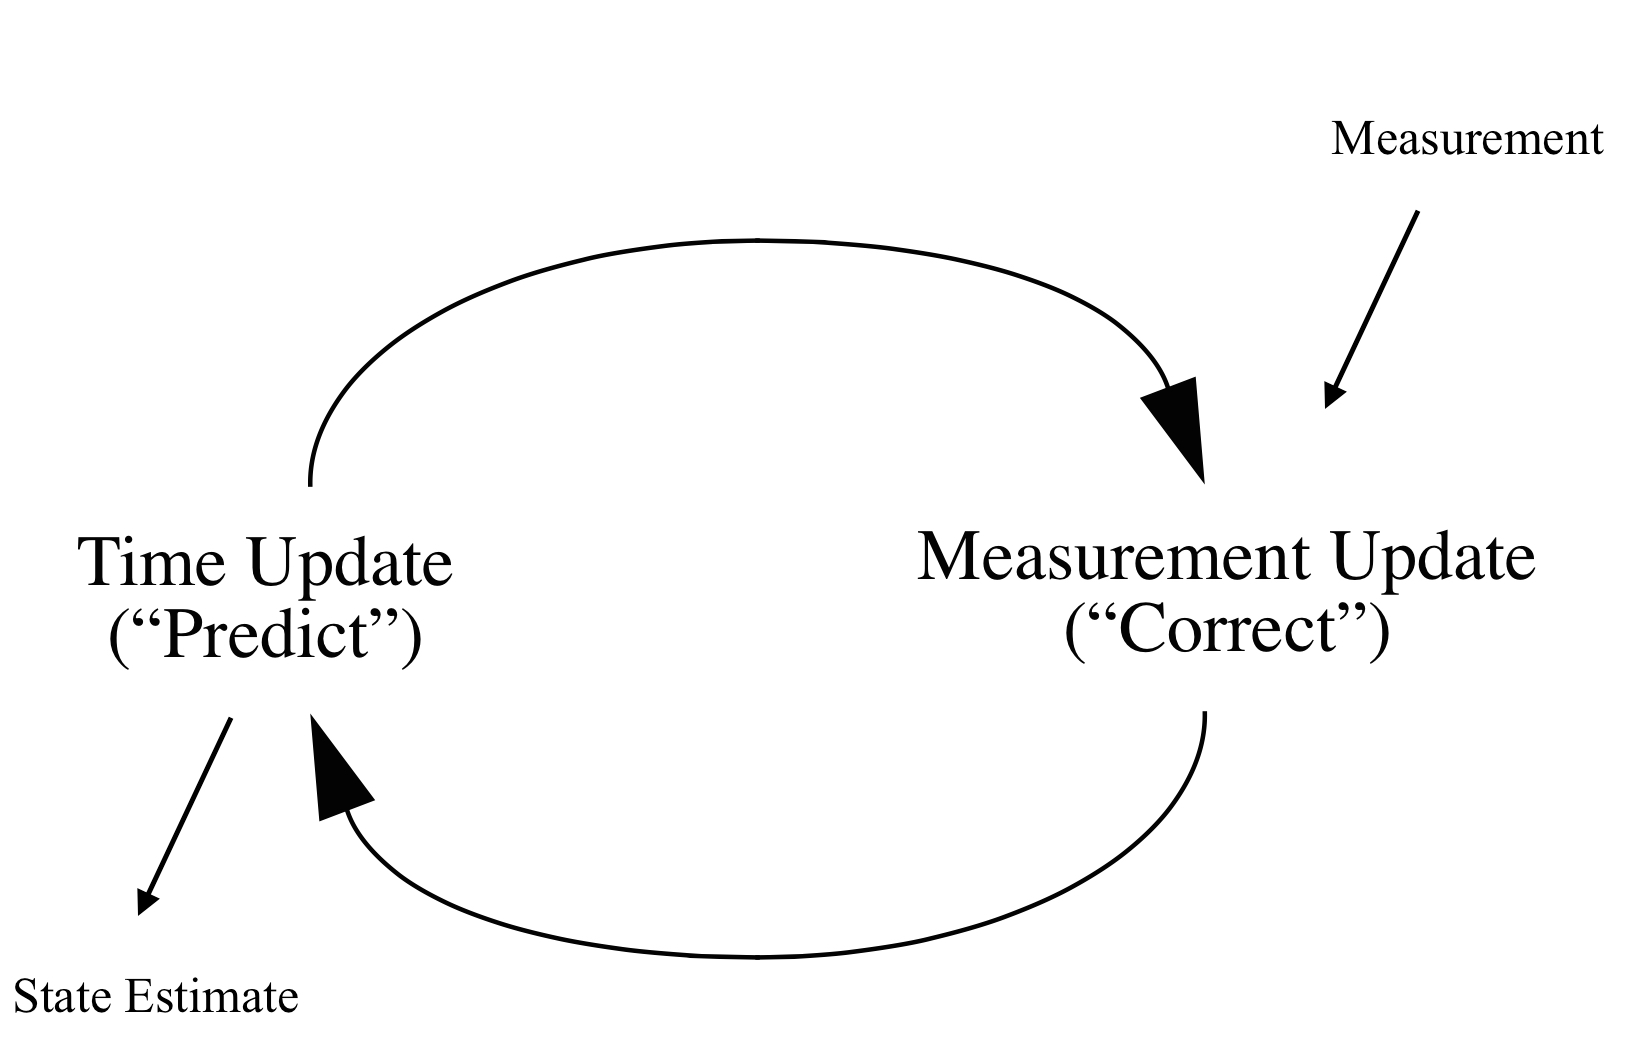
\includegraphics[width = 0.7\textwidth]{Kalmanphasepic.jpg}
\caption{Kalman phases.}
\label{figure : Kalman phases}
\end{figure}

During the \textit{predict} phase the filter estimates the states using the inputs from the process, i.e the gyroscope. \ref{figure : Kalman phases}
\begin{equation}
\hat{x^-_k} = A\hat{x}^-\textsubscript{k-1}+Bu\textsubscript{k-1}
\end{equation}
As stated above \textbf{För slentriant?} the Kalman filter uses readings from both the gyro and accelerometer to estimate a position closer to the true value. To determine how reliable the process and measurement readings are a noise covariance is defined as
\begin{equation} \label{eq:covariance process noise}
Q = E(w_k w_k \textsuperscript{T})
\end{equation}
\begin{equation} \label{eq:covariance measurement noise}
R = E(z_k z_k \textsuperscript{T} )
\end{equation}
From here a \textit{priori} error covariance matrix is introduced to symbolize the noise in the process measurement.
\begin{equation}
P^-_k = AP^-1\textsubscript{k-1}A^T + Q_k
\end{equation}
During the \textit{update} the accelerometer values are used. The measurement \textit{innovation} is calculated as
\begin{equation}
\tilde{y} = z_k - H\hat{x}^-_k
\end{equation}
The \textit{innovation} is a residual that reflects the relation between the predicted measurement and the actual measurement. A measurement \textit{innovation} of zero indicates a perfect agreement.
The measurement \textit{innovation} covariance is calculated as
\begin{equation}
S_k = HP^-_kH^T + R
\end{equation}
This is very similiar to the \textit{priori} error covariance but represents the measurement instead. From here the core of the Kalman filter can be calculated, the Kalman gain
\begin{equation}
K_k = P^-_kH^TS\textsuperscript{-1}_k
\end{equation}
indicates how reliable the measurement is. Note that if the measurement covariance error \eqref{eq:covariance measurement noise} is large the Kalman gain will be small and the opposite if the\textit{priori} error covariance is large \textbf{superlång mening ?}.
By now the \textit{posteriori} state can be estimated by
\begin{equation}
\hat{x}_k = \hat{x}^-_k + K_k\tilde{y}_k
\end{equation}
A current state has been estimated and the Kalman filter returns to the measurement phase seen in figure \ref{figure : Kalman phases}.
For further reading, and mathematical proof see \cite{Kalmanintro}.

 
\chapter{Demonstrator}
\emph{Detta kapitel beskriver både den utvecklade demonstratorn och den aktuella arbetsprocessen som demonstartorn utvecklats enligt, dvs resultatet och vägen dit.}


\section{Problem Formulation}
%Beskriv din problemställning för demonstratorn.\\

The engineering problem were to build a cube that, using a reaction wheel, could balance on its edge.
\emph{To be continued}
\section{State space model}
PICTURE TO BE ADDED
\\
To create a state-space model the physical model has to be translated to a mathematical model. The system can be estimated much like an inverted pendulum as a two-degree-of-freedom model \ref{KTHpendulum}. \emph{Lagrangian} Dynamics can be used to derive the systems behaviour. Firstly by expressing the generlized forces, the energy functions and lagrangian. And then acquire the equations of motion with the Lagrange equation \ref{Lagrangeswing}.
\begin{equation}
Q_i=\frac{d}{dt}\left(\frac{\partial L}{\partial \dot{q_i}}\right)-\left(\frac{\partial L}{\partial q_i}\right)
\end{equation}
In this case the cube's angular momentum is counteracted by the flywheel and the system can be written as follows

%\begin{equation}
\begin{equation} \label{eq:positiveL}
M_a=\frac{d}{dt}\left(\frac{\partial L}{\partial \dot{\theta}}\right)-\left(\frac{\partial L}{\partial \theta}\right)
\end{equation}
\begin{equation} \label{eq:negativeL}
-M_a=\frac{d}{dt}\left(\frac{\partial L}{\partial \dot{\phi}}\right)-\left(\frac{\partial L}{\partial \phi}\right)
\end{equation}
Whereas $\theta$ represents the angle of the cube and $\phi$ is the position of the flywheel. \\
The Lagrange equation is derived from the difference in kinetic energy and potential energy of the cube
\begin{equation} \label{eq:Lagrange}
L = E_k - E_p
\end{equation}

\begin{equation}
E_k = \frac{I_c \cdot \dot{\theta^2}}{2} + \frac{I_f \cdot \dot{\phi^2} }{2}
\end{equation}
\begin{equation}
E_p = \frac{M_c \cdot g \cdot l \cdot \cos \theta}{\sqrt{2}}
\end{equation}
Equation \eqref{eq:positiveL} and \eqref{eq:negativeL} with \eqref{eq:Lagrange}
\begin{equation} \label{eq:negativeL2}
I_k \cdot \ddot{\theta} - \frac{M_c \cdot g \cdot l \cdot \sin \theta }{\sqrt{2}}  = -M_a
\end{equation}
\begin{equation} \label{eq:postiveL2}
I_s \cdot \ddot{\phi} = M_a
\end{equation}
From these equations it is evident that $M_a$ is the torque executed by the flywheel which is wielded by the motor torque $\tau$, it can be described by a relation between the torque constant and the current flowing through the motor.
\begin{equation}
\tau = K_t \cdot i_m
\end{equation}
The current can be described by the voltage across the two poles of the motor. 
\begin{equation}
\tau = K_t \cdot \frac{U-E_{\text{emf}} }{R_m}
\end{equation}
\textbf{Mention that inductance is neglected due to something? see KTHpendulum reference}
The induced voltage is related to the induced voltage constant and the rotor rotation
\begin{equation}
E_{\text{emf}} = K_{\text{emf}} \cdot \dot{\phi_r}
\end{equation}
\begin{equation}
\phi_r = \dot{\phi} - \dot{\theta}
\end{equation}
 
\begin{equation} \label{eq:tau}
\tau = \frac{K_t}{R_m} U - \frac{K_t K_{\text{emf}} }{R_m} \dot{\phi} + \frac{K_t K_{\text{emf}} }{R_m} \dot{\theta}
\end{equation}
The torque on the executed by the flywheel can then be described with the efficiency of the motor
\begin{equation} \label{eq:eff}
M_a = \tau \cdot \eta_m
\end{equation}
Based on equation \eqref{eq:negativeL}, \eqref{eq:positiveL} and \eqref{eq:eff} the system can be described by
\begin{equation}
\ddot{\theta} = -\frac{K_t \eta_m}{R_m I_c} U + \frac{K_t K_{\text{emf}} \eta_m}{R_m I_c} \dot{\phi} - \frac{K_t K_{\text{emf}} \eta_m}{R_m I_c} \dot{\theta} + \frac{Mt g l }{\sqrt{2} I_c} \sin \theta \label{thetadotdot}
\end{equation}
\begin{equation}
\ddot{\phi} = \frac{K_t \eta_m}{R_m I_f} U + \frac{K_t K_{\text{emf}} \eta_m}{R_m I_f} \dot{\phi} - \frac{K_t K_{\text{emf}} \eta_m}{R_m I_f} \dot{\theta} 
\label{phidotdot}
\end{equation} 
With the equations \eqref{thetadotdot} and \eqref{phidotdot} the system can be described with a state space model with a states $x^T = [\theta, \dot{\theta}, \dot{\phi}$]. The system is hence described by
\begin{equation}
\dot{x} = Ax + Bu
\end{equation} 
where \\
\begin{center}
$A =\begin{bmatrix}
0 & 1 & 0 \\
\dfrac{Mt g l }{\sqrt{2} I_c} & - \dfrac{K_t K_{\text{emf}} \eta_m}{R_m I_c} & \dfrac{K_t K_{\text{emf}} \eta_m}{R_m I_c} \\ 
0 & \dfrac{K_t K_{\text{emf}} \eta_m}{R_m I_f} & -\dfrac{K_t K_{\text{emf}} \eta_m}{R_m I_f}
\end{bmatrix}$

$B = \begin{bmatrix}
0 \\ 
-\dfrac{K_t \eta_m}{R_m I_c} \\
\dfrac{K_t \eta_m}{R_m I_f}
\end{bmatrix} $
\end{center}

\section{Discrete Kalman filter} \label{sec: discrete kalman}
To implement the Kalman filter in algorithm it has to be discretizied 
This is done much like a feedback control. The filter firstly? estimates the process state and then obtains feedback as noisy measurements. That means that the filter works in two steps, a \textit{time update} and a \textit{measurement update}. The names implicate that the \textit{time update} projects the next state to obtain the \textit{priori estimate} whilst the \textit{measurement update} uses the feedback mentioned above to obtain an improved \textit{posteriori} estimate.
\textbf{We need a picture here, but not the same as david and viktor...}

Some of the implementation and discretization of the filter.
\subsection{Kalman implementation}
An implementation of the Kalman filter on the IMU would look something like this for the gyroscope
\begin{equation}
\theta_k = \theta \textsubscript{k-1} + (w_k \mp b\textsubscript{k-1}) \Delta t
\end{equation}
\begin{equation}
b_k = b\textsubscript{k-1}
\end{equation}
\begin{equation}
z_k = a_k
\end{equation}
With $b$ as the gyro bias
Looking at equation \eqref{eq:kalmanstate} the system can be written
\begin{equation}
\textbf{x}_k = \begin{bmatrix}
\theta \\
\dot{\theta_b}_k
\end{bmatrix}
\end{equation}

\begin{equation}
\textbf{A} = \begin{bmatrix}
1  & -\Delta t \\
0   & 1
\end{bmatrix}
\end{equation}

\begin{equation}
\textbf{B} = \begin{bmatrix}
\Delta t \\ 0
\end{bmatrix}
\end{equation}


\begin{figure}[!htb]
\centering
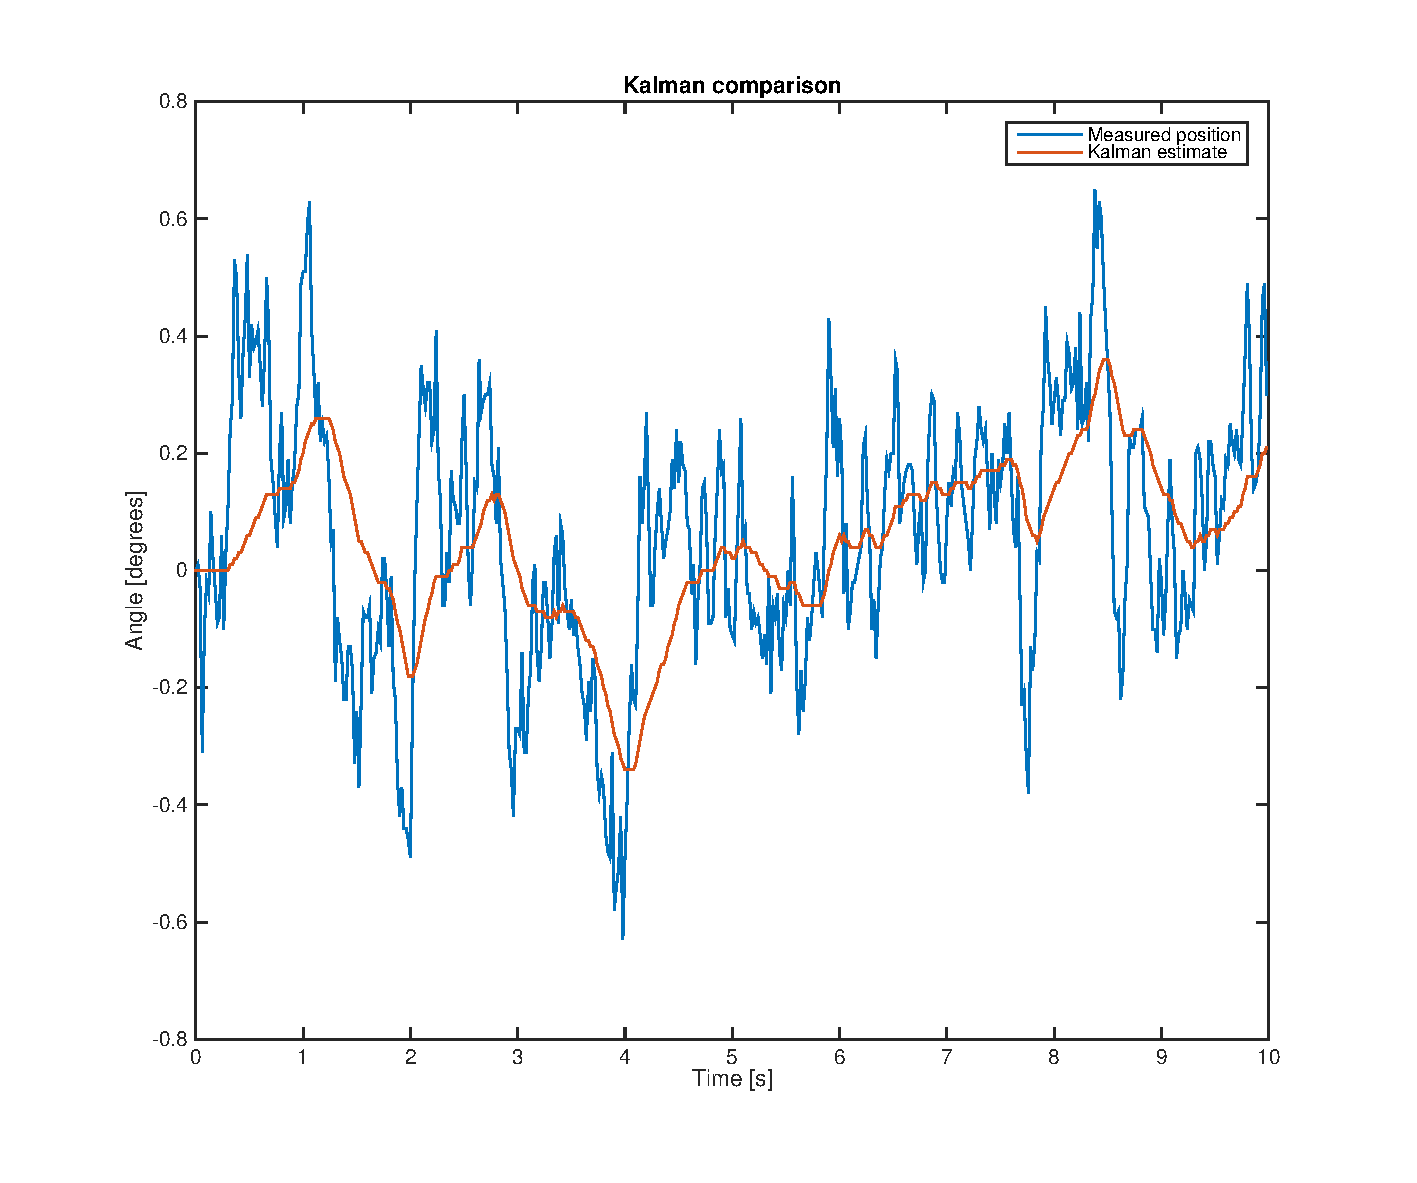
\includegraphics[scale=.7]{Kalmancomparisonplot.eps}
\caption{Comparison of Kalman filtered signal and original signal}
\label{fig:Kalman comparison}
\end{figure}



\subsection{Error thingys}
For the Kalman filter to properly work it is essential to know how reliable the process and measurement input is. A way of determining the process noise and measurement noise of the IMU is the Allan variance method \ref{AllanV}.
The gyro data is treated as an external input the system, so the error and bias from the gyro readings are characterised as process noise. The advantage of using the gyro data instead of accelerometer data is the reduction in states as the accelerometer would need to be integrated twice to retrieve and angle ( elaborate....)

\section{Software}
To develop and improve a system such as this is an iterative process. To verify changes and improvements in realtime Simulink\textsuperscript{\textregistered} was used togheter with the mathematical model. 
%\begin{figure}[!htb]
%\centering
%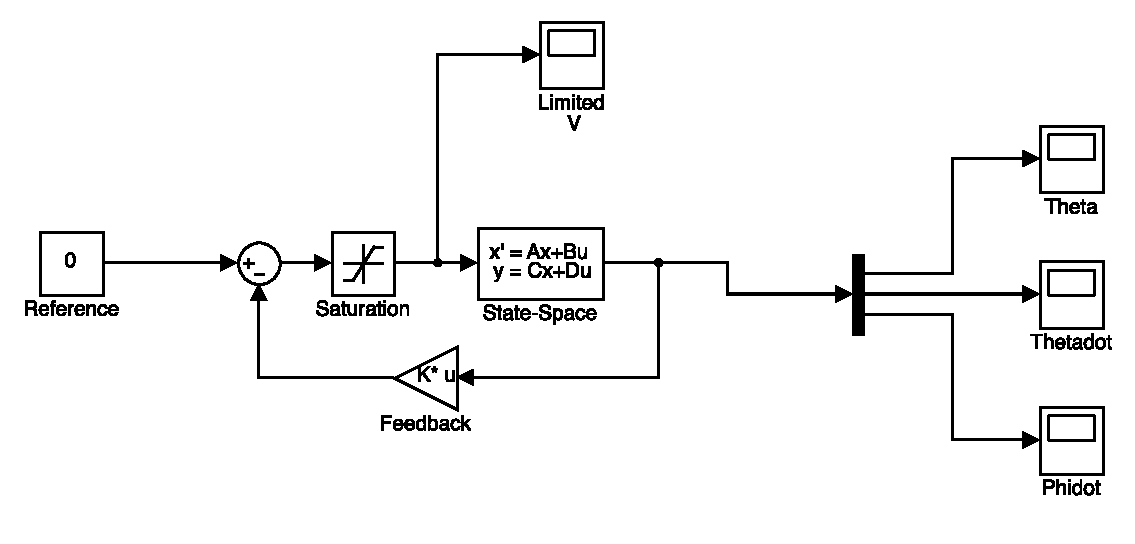
\includegraphics[scale=.7]{simmodel.eps}
%\caption{Simulink model.}
%\label{fig:simmodel}
%\end{figure}



The Simulinkmodel seen in figure \ref{fig:simmodel} describes the system
\\ Something about the  optimizing of the feedback control
\begin{figure}[!htb]
\centering
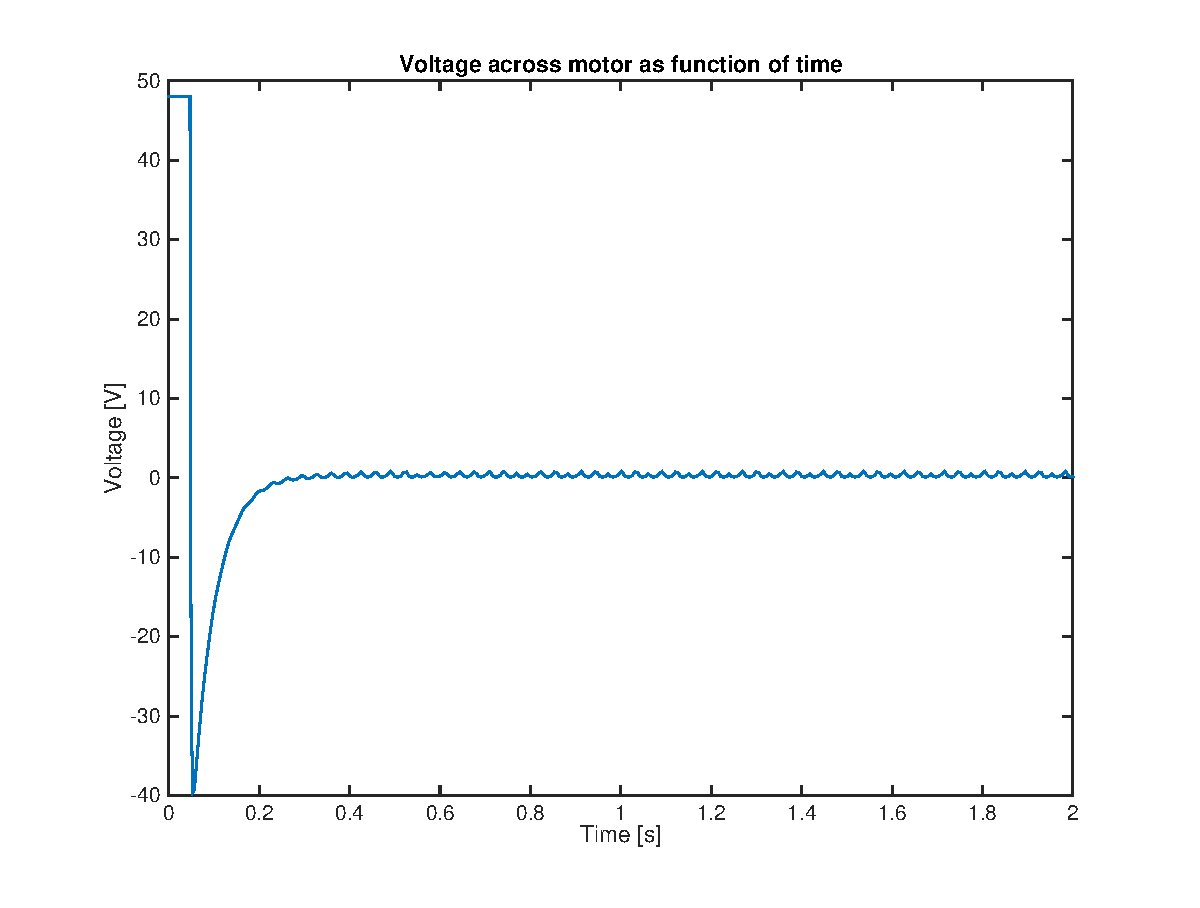
\includegraphics[scale=.7]{voltageplot.eps}
\caption{Voltage across motor poles.}
\label{fig:voltageplot}
\end{figure}

The voltage supplied to the motor

\begin{figure}[!htb]
\centering
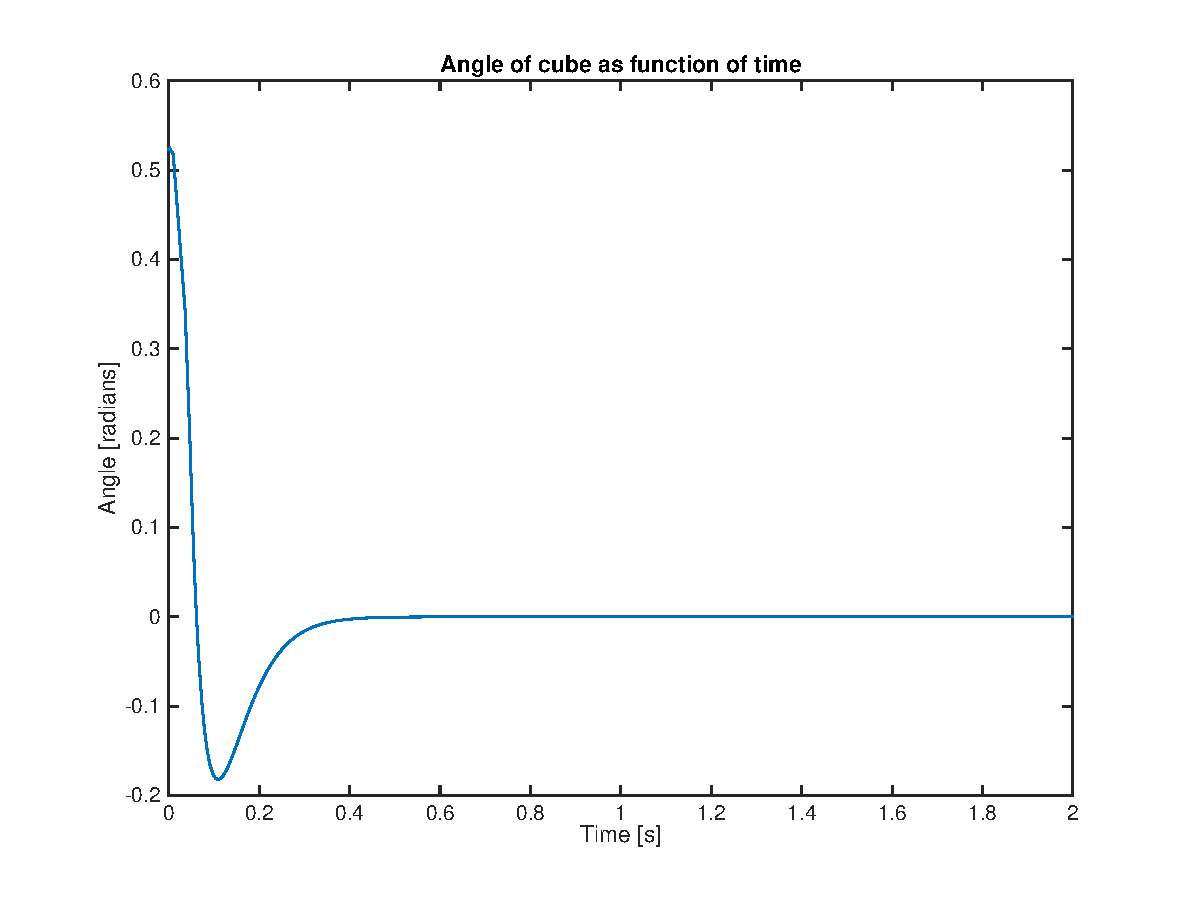
\includegraphics[scale=.7]{angleplot.eps}
\caption{Angle of the cube.}
\label{fig:voltageplot}
\end{figure}

The angle of the cube. Very good such magic


\section{Electronics}
Beskriv din elektroniska konstruktion. Använd figurer och förenklade blockschema. Motivera dina lösningar.
How do we send data?
\\ Sensors
\\ Motor
\\ Arduino
\\ Motor control


\section{Hardware}
The motor is fixed through the middle wall in the cube, the shaft on one side and the body on the other. The flywheel is dicrectly mounted to the motor shaft. All other components are mounted on the motor-body side of the cube.
\\ Basic construction

\section{Results}
Beskriv resultatet.


\chapter{Discussion and conclusions}
\emph{I detta kapitel diskuteras och sammanfattas de resultat som presenterats i föregående kapitel. Sammanfattningen baseras på en resultatanalys och syftar till att svara på den fråga eller de frågor som formuleras i kapitel i.}

\section{Discussion}
Motor choice osv

\section{Conclusions}
Successful victory


\chapter{Recommendations and future work}

\section{Recommendations}
A more extensive research with non-linear control systems has been done at ETH, with the name Cubli,\cite{cubliECC13}

\section{Future work}
An extension of the project would be balancing the cube not only on it's edge but it's corner. To achieve this multiple reaction wheels must be used and a more complicated control system due to changes in moment of inertia caused by angular velocities in the other reaction wheels.

%\bibliography
\cleardoublepage
\bibliography{FiM_references}
\bibliographystyle{elsarticle-num-names}%apalike-url}

\cleardoublepage
\appendix
\addtocontents{toc}{\protect\contentsline {part}{Appendices}{}{}}


\chapter{Additional information} \label{appA}

\chapter{Proofs} \label{appB}

\cleardoublepage   
\cleartoverso %force back cover to be "left" page
%
\includepdf[pages={2}]{kth-cover.pdf}

%\printbibliography
\end{document}

